\documentclass[aspectratio=169, 11pt]{beamer}

% ── Theme & Colors ──────────────────────────────────────────
\usetheme{Madrid}
\usecolortheme{default}

\definecolor{darkcharcoal}{HTML}{2C3E50}
\definecolor{accentblue}{HTML}{2980B9}
\definecolor{donegreen}{HTML}{27AE60}
\definecolor{pendinggray}{HTML}{BDC3C7}
\definecolor{lightbg}{HTML}{F8F9FA}
\definecolor{darktext}{HTML}{1A1A2E}

\setbeamercolor{structure}{fg=darkcharcoal}
\setbeamercolor{palette primary}{bg=darkcharcoal, fg=white}
\setbeamercolor{palette secondary}{bg=accentblue, fg=white}
\setbeamercolor{frametitle}{bg=darkcharcoal, fg=white}
\setbeamercolor{title}{fg=darkcharcoal}
\setbeamercolor{subtitle}{fg=accentblue}
\setbeamercolor{block title}{bg=darkcharcoal, fg=white}
\setbeamercolor{block body}{bg=lightbg, fg=darktext}
\setbeamercolor{item}{fg=accentblue}

\setbeamertemplate{navigation symbols}{}
\setbeamerfont{frametitle}{size=\large, series=\bfseries}
\setbeamerfont{title}{size=\Large, series=\bfseries}

% ── Packages ────────────────────────────────────────────────
\usepackage{tikz}
\usetikzlibrary{shapes.geometric, arrows.meta, positioning, fit, calc}
\usepackage{amsmath, amssymb}
\usepackage{booktabs}
\usepackage{graphicx}
\usepackage{hyperref}
\usepackage{xcolor}
\usepackage{array}

% ── TikZ Styles ─────────────────────────────────────────────
\tikzstyle{block} = [rectangle, rounded corners, minimum width=2.2cm, minimum height=0.8cm, text centered, draw=darkcharcoal, fill=lightbg, font=\small]
\tikzstyle{done} = [block, draw=donegreen, fill=donegreen!10, text=donegreen!80!black]
\tikzstyle{pending} = [block, draw=pendinggray, fill=pendinggray!15, text=pendinggray!60!black]
\tikzstyle{arrow} = [-{Stealth[length=2.5mm]}, thick, color=darkcharcoal!70]

% ── Meta ────────────────────────────────────────────────────
\title{Optimising Fed-Batch Feed-Flow Strategies}
\subtitle{UG Project Progress Report --- VIIth Semester}
\author{Yashashwi Singhania}
\date{July 2026}

% ═══════════════════════════════════════════════════════════
\begin{document}

% ── Slide 1: Title ──────────────────────────────────────────
\begin{frame}[plain]
  \vfill
  \begin{center}
    
\includegraphics[height=2.2cm]{iit_bhu_logo.png}\\[0.5cm]
    {\Large\bfseries\color{darkcharcoal} Indian Institute of Technology (BHU), Varanasi}\\[0.6cm]
    {\LARGE\bfseries\color{darkcharcoal} Optimising Fed-Batch}\\[0.15cm]
    {\LARGE\bfseries\color{darkcharcoal} Feed-Flow Strategies}\\[0.4cm]
    {\large\color{accentblue} BC-XXX : UG Project - 2 Semester Report}\\[0.8cm]
    \begin{tabular}{rl}
      \textbf{Student:} & Yashashwi Singhania (23014019) \\
      \textbf{Guide:} & Dr.\ Sharon Mano Pappu J. \\
      \textbf{Department:} & Biochemical Engineering \\
      \textbf{Lab:} & Bioprocess Development and Digitalization Laboratory \\
    \end{tabular}\\[0.5cm]
    {\small July 2026}
  \end{center}
  \vfill
\end{frame}

% ── Slide 2: Recap + This Semester ──────────────────────────
\begin{frame}{Recap and This Semester's Progress}
  \begin{block}{Where we left off (VIth semester)}
    Surveyed 9 literature products' $q_p$--$\mu$ relationships (linear, bell-shaped,
    hyperbolic), fitted them, and simulated batch X/S/P dynamics. The theory predicted
    a feeding rule per shape --- but never tested it quantitatively.
  \end{block}

  \vspace{0.3cm}
  \begin{columns}[T]
    \begin{column}{0.48\textwidth}
      \textbf{This Semester --- Completed:}
      \begin{itemize}
        \item[\textcolor{donegreen}{\checkmark}] Built a fed-batch (F(t)) process model for all 9 products
        \item[\textcolor{donegreen}{\checkmark}] Implemented \& optimised 7 feed-flow strategies
        \item[\textcolor{donegreen}{\checkmark}] Found \& fixed a working-volume ceiling bug
        \item[\textcolor{donegreen}{\checkmark}] Fixed a pygmo/FastAPI threading crash in the web backend
      \end{itemize}
    \end{column}
    \begin{column}{0.48\textwidth}
      \textbf{Next Steps:}
      \begin{itemize}
        \item[\textcolor{pendinggray}{$\circ$}] Port the model into real \texttt{pyfoomb.BioprocessModel}
        \item[\textcolor{pendinggray}{$\circ$}] Re-optimise with \texttt{Caretaker.estimate\_parallel()} (pygmo)
        \item[\textcolor{pendinggray}{$\circ$}] Validate winning strategies against real fed-batch data
        \item[\textcolor{pendinggray}{$\circ$}] Add feed-flow optimisation as a GUI page
      \end{itemize}
    \end{column}
  \end{columns}
\end{frame}

% ── Slide 3: Control chain + theory ─────────────────────────
\begin{frame}{From Theory to a Testable Question}
  \begin{block}{The control chain established last semester}
    \centering
    $F(t) \;\rightarrow\; D = F/V \approx \mu \;\rightarrow\; q_p(\mu) \;\rightarrow\; P$
  \end{block}

  \vspace{0.3cm}
  \begin{center}
  \renewcommand{\arraystretch}{1.3}
  \begin{tabular}{ll}
    \toprule
    \textbf{$q_p(\mu)$ shape} & \textbf{Theoretical feeding rule} \\
    \midrule
    Linear (Luedeking--Piret) & push $\mu$ as high as the data supports \\
    Bell-shaped (Gaussian) & hold $\mu$ at exactly $\mu_{opt}$ \\
    Hyperbolic (saturating) & any $\mu$ comfortably above $K_\mu$ is fine \\
    \bottomrule
  \end{tabular}
  \end{center}

  \vspace{0.3cm}
  \textbf{This semester's question:} does this qualitative rule actually hold when
  7 concrete feed-flow functions $F(t)$ compete head-to-head, under a shared,
  realistic reactor budget?
\end{frame}

% ── Slide 4: Process model ──────────────────────────────────
\begin{frame}{Process Model}
  Every one of the 9 datasets runs in the \textbf{same generic reactor}, so only the
  $q_p(\mu)$ \textit{shape} (and the organism's own $\mu_{max}/K_S/Y_{X/S}$) differs
  between runs.

  \vspace{0.2cm}
  \begin{columns}[T]
    \begin{column}{0.46\textwidth}
      \textbf{Batch phase} ($F=0$):\\
      {\small $X_0$=0.1 g/L, $S_0$=20 g/L, $V_0$=1 L, Monod kinetics until $S$ depletes
      to 0.5 g/L --- when the feed pump switches on.}
    \end{column}
    \begin{column}{0.5\textwidth}
      \textbf{Fed-batch phase} (fixed 40 h horizon):
      \begin{align*}
        \dot X &= \mu X - (F/V)X \\
        \dot S &= (F/V)(S_{in}-S) - (\mu/Y_{X/S})X \\
        \dot P &= q_p(\mu) X - (F/V)P \\
        \dot V &= F,\qquad \mu = \mu_{max}\tfrac{S}{K_S+S}
      \end{align*}
    \end{column}
  \end{columns}

  \vspace{0.15cm}
  {\small Shared feed reservoir $S_{in}=400$ g/L, working-volume ceiling $V_{max}=4$ L
  (4$\times$ fill), feed-pump cap $F_{cap}=2$ L/h. Integrated with
  \texttt{solve\_ivp(LSODA)}.}
\end{frame}

% ── Slide 5: Seven feed-flow strategies ─────────────────────
\begin{frame}{Seven Feed-Flow Strategies}
  {\small Each strategy's free parameters are optimised with
  \texttt{scipy.optimize.differential\_evolution} --- the same global,
  derivative-free family pyFOOMB's own \texttt{Caretaker.estimate()} uses.}

  \vspace{0.2cm}
  \begin{center}
  \renewcommand{\arraystretch}{1.2}
  {\footnotesize
  \begin{tabular}{lll}
    \toprule
    \textbf{Strategy} & \textbf{$F(t)$} & \textbf{Free parameters} \\
    \midrule
    Constant & $F_0$ & $F_0$ \\
    Exponential & $F_0 e^{\mu_{set} t}$ & $F_0, \mu_{set}$ \\
    Linear ramp & $F_0 + kt$ & $F_0, k$ \\
    Exponential + linear & $F_0 e^{\mu_{set} t} + kt$ & $F_0, \mu_{set}, k$ \\
    Two-stage & $F_1$ until $t_{switch}$, then $F_2$ & $F_1, F_2, t_{switch}$ \\
    Pulsed & square wave, period $T_{cycle}$, duty cycle & $F_{pulse}, T_{cycle}, \text{duty}$ \\
    Feedback control & $K_p(S_{set}(\mu_{target}) - S(t))$, clipped $\geq 0$ & $\mu_{target}, K_p$ \\
    \bottomrule
  \end{tabular}
  }
  \end{center}

  \vspace{0.2cm}
  {\small ``Exponential + linear'' generalises both pure exponential and pure
  linear-ramp ($k{=}0$ or $\mu_{set}{=}0$ recovers them) --- added to test whether
  combining ``hold a growth rate'' with ``keep adding a little extra'' ever wins.
  Objective: maximise total product $P(t_f)\cdot V(t_f)$.}
\end{frame}

% ── Slide 6: A bug found along the way ──────────────────────
\begin{frame}{A Bug Found Along the Way: Volume-Ceiling Enforcement}
  \begin{columns}[T]
    \begin{column}{0.48\textwidth}
      \textbf{The problem:}
      \begin{itemize}
        \item $V \leq V_{max}$ was enforced only as a \textbf{soft quadratic penalty}
              in the DE objective.
        \item The penalty barely bites right at the boundary.
        \item Checked against the first committed sweep: \textbf{57 of 63 optimised
              runs ended with $V_{final} > V_{max}$} (median +0.7\%, worst case +8.6\%).
      \end{itemize}
      Most ``winning strategies'' came from a search space that overflows the
      reactor it claims to model.
    \end{column}
    \begin{column}{0.48\textwidth}
      \textbf{The fix:}
      \begin{itemize}
        \item Clip the feed to zero once $V \geq V_{max}$ \textbf{inside the ODE
              right-hand side itself}, not via a penalty.
        \item Same as a real fed-batch: the pump physically stops at a full vessel.
        \item Re-verified: $V_{final}$ now lands at $4.0000$--$4.0001$ L (numerical
              tolerance only) instead of overshooting to $4.34$ L.
      \end{itemize}
      \vspace{0.2cm}
      \begin{block}{}
        \small The full 63-run sweep was re-run after this fix --- results on the
        following slides reflect the \textbf{corrected}, volume-respecting numbers.
      \end{block}
    \end{column}
  \end{columns}
\end{frame}

% ── Slide 7: Results table (placeholder -- filled after rerun) ──
\begin{frame}{Winner Per Dataset (7 Strategies)}
  \vspace{-0.1cm}
  {\small Winning feed-flow strategy per product, after the volume-ceiling fix:}

  \vspace{0.2cm}
  \begin{center}
  \renewcommand{\arraystretch}{1.15}
  {\footnotesize
  \begin{tabular}{llccc}
    \toprule
    \textbf{$q_p(\mu)$ shape} & \textbf{Product} & \textbf{Winning strategy} & \textbf{Margin} & \textbf{Spread} \\
    \midrule
    %RESULTS_TABLE%
    \bottomrule
  \end{tabular}
  }
  \end{center}

  \vspace{0.15cm}
  {\small Margin = \% more product than the runner-up. Spread = \% more product than
  the worst strategy, for that dataset.}
\end{frame}

% ── Slide 8: Strategy comparison figure ─────────────────────
\begin{frame}{Strategy Comparison: Total Product per Dataset}
  \vfill
  \begin{center}
    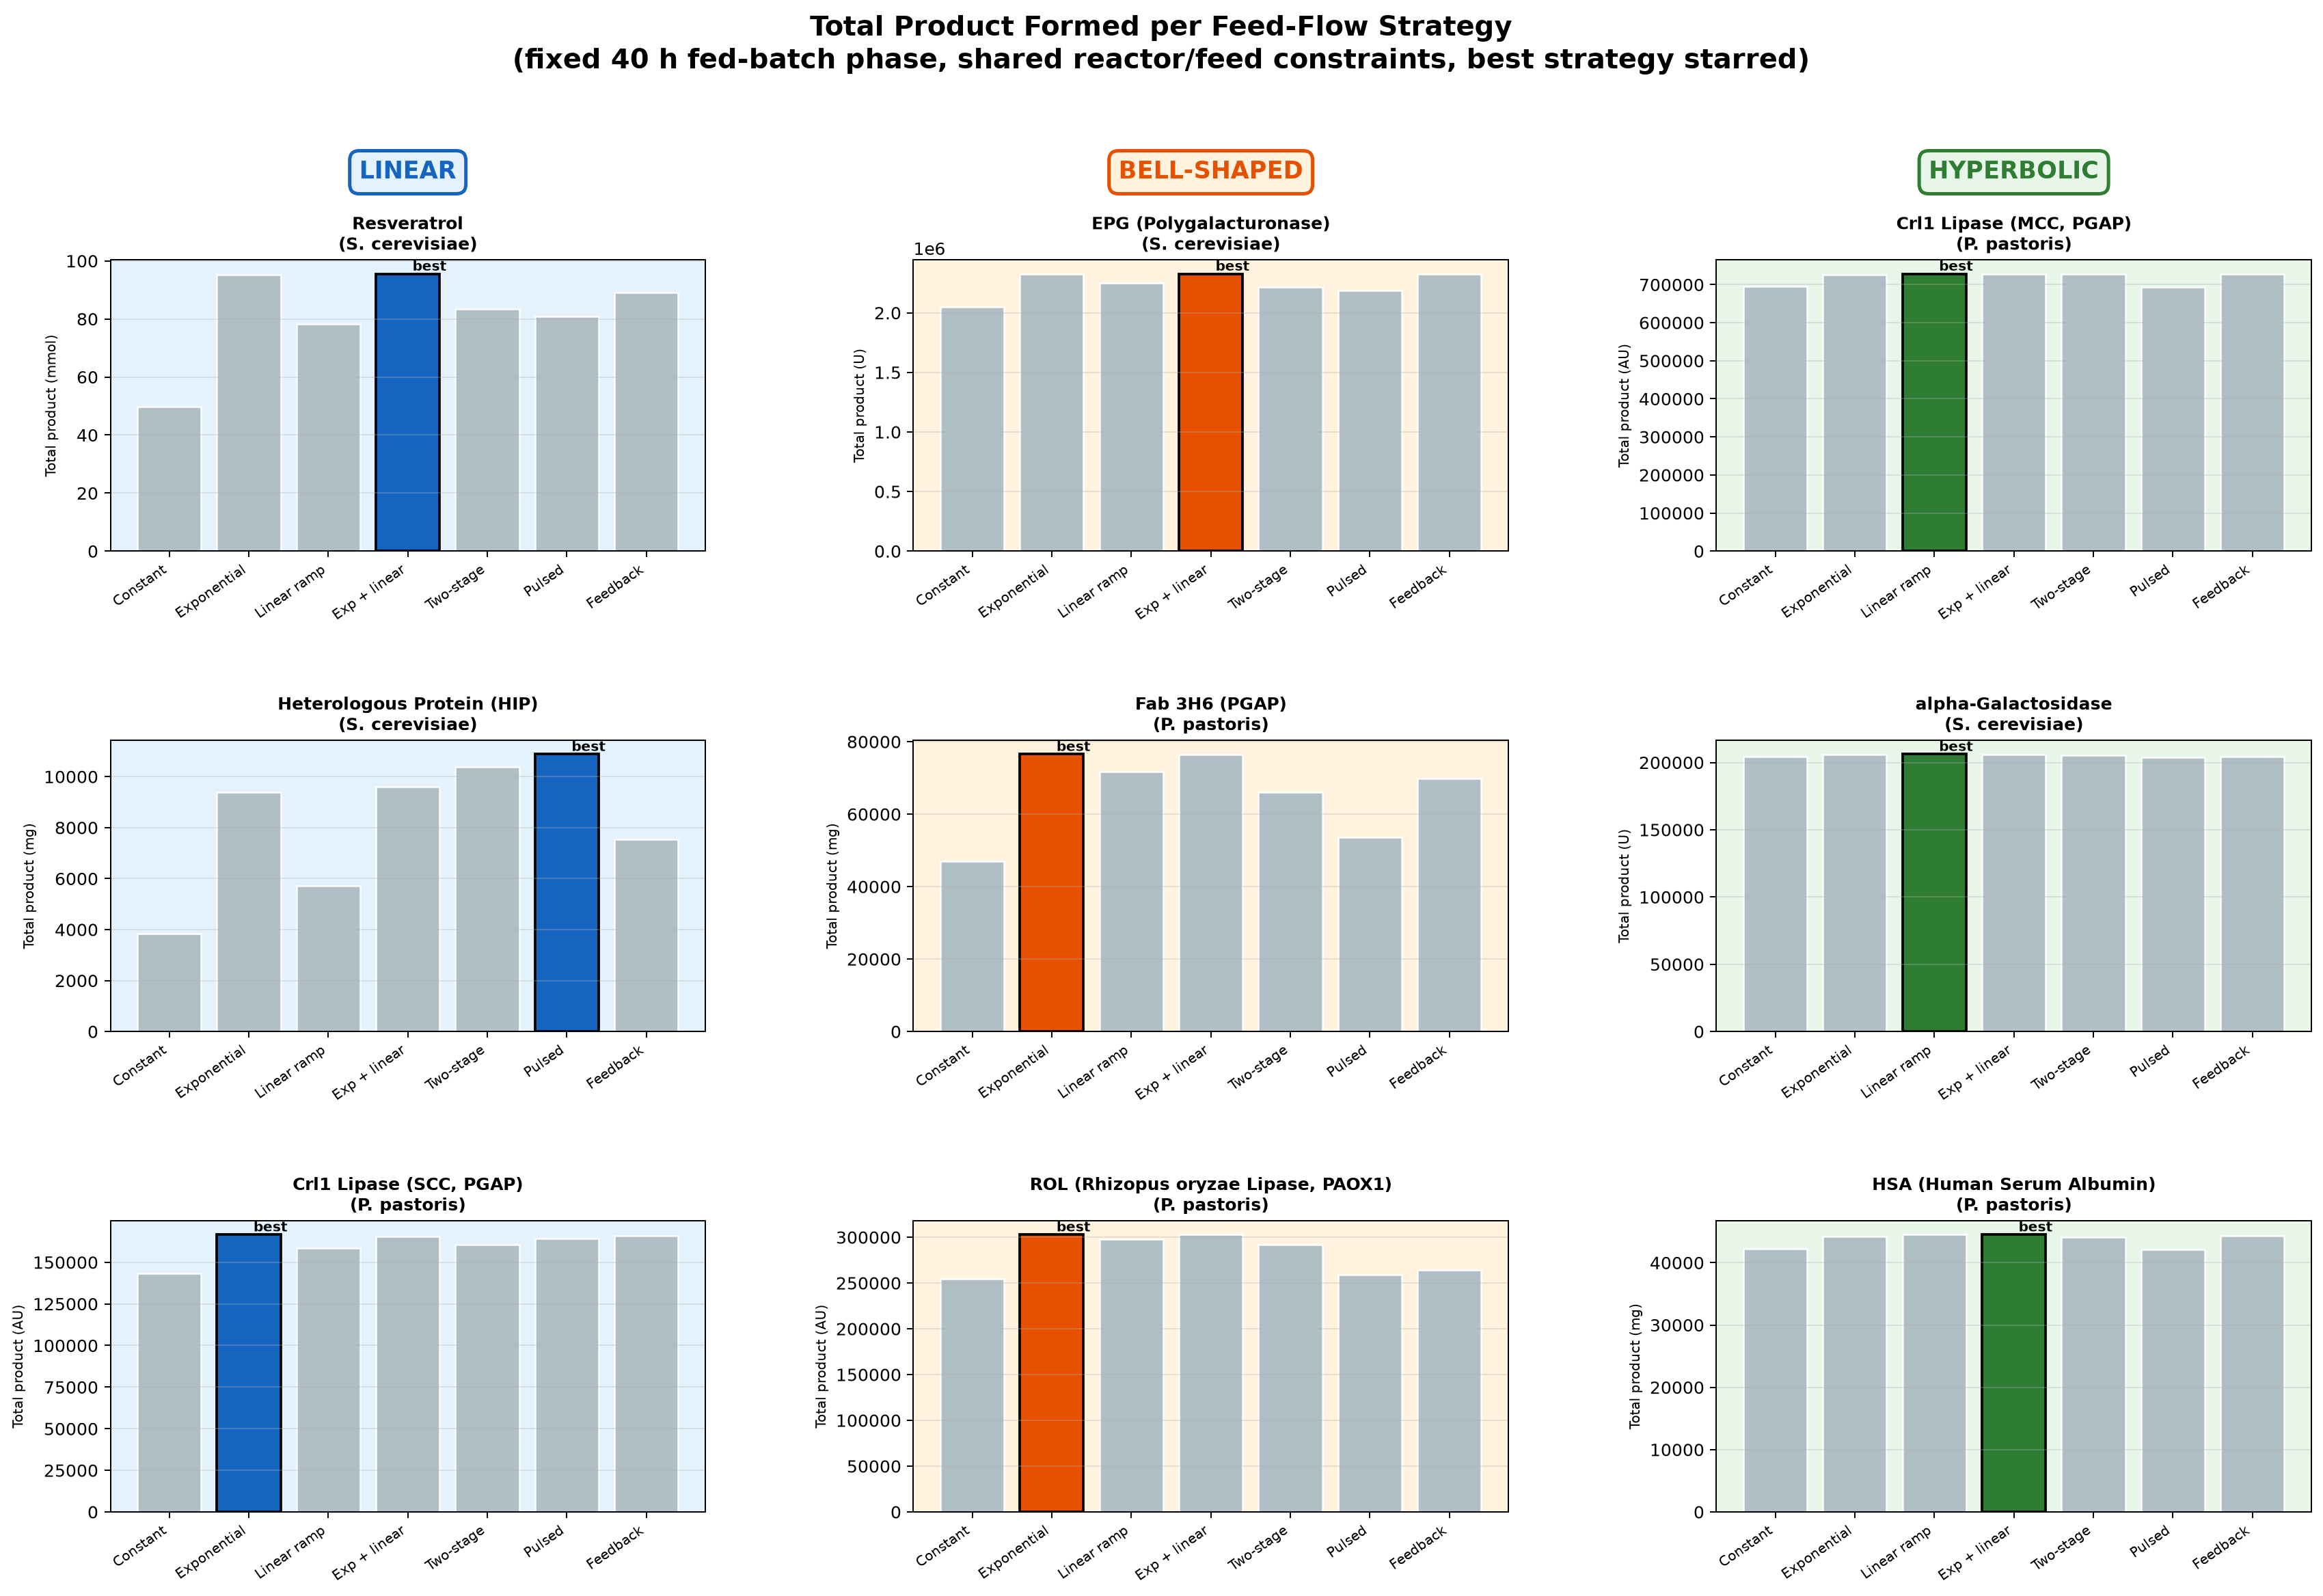
\includegraphics[height=0.82\textheight]{feed_flow_strategy_comparison.png}
  \end{center}
  \vfill
\end{frame}

% ── Slide 9: Best profiles figure ───────────────────────────
\begin{frame}{Winning Strategy Time-Courses}
  \vfill
  \begin{center}
    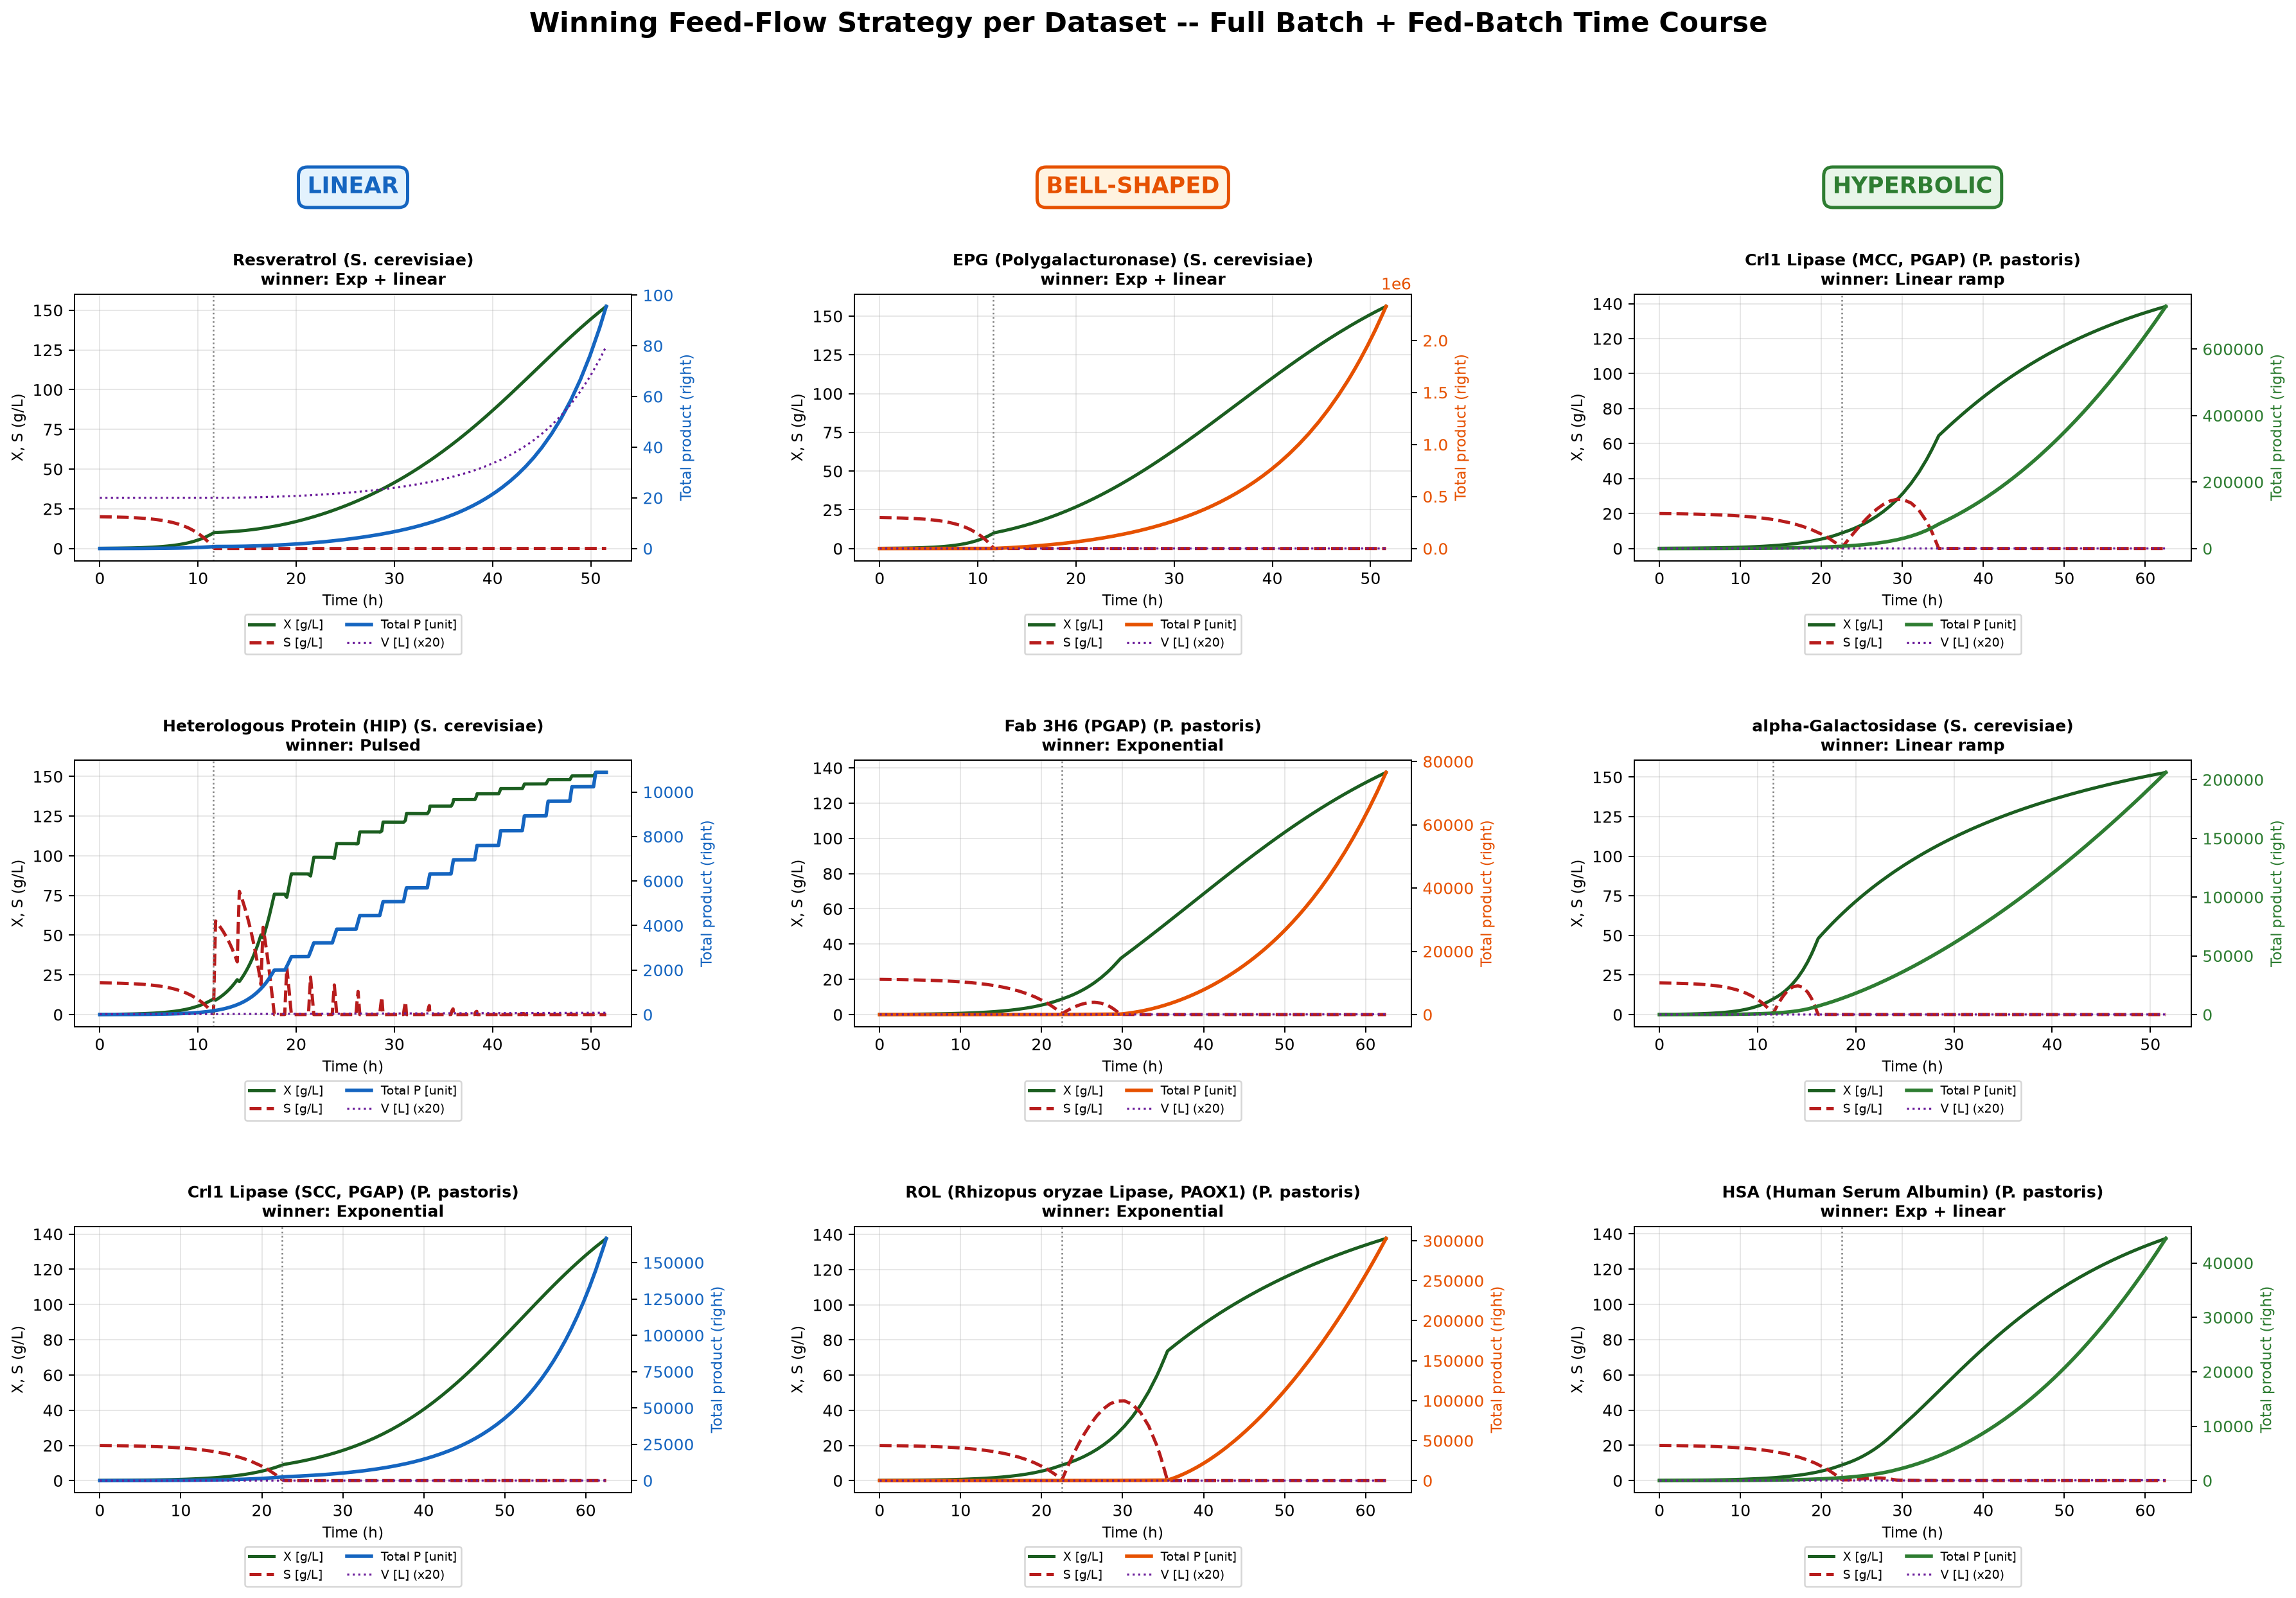
\includegraphics[height=0.82\textheight]{feed_flow_best_profiles.png}
  \end{center}
  \vfill
\end{frame}

% ── Slide 10: Linear-ramp-only figure ───────────────────────
\begin{frame}{A Simple, Practical Baseline: Linear-Ramp Feeding}
  {\small A single, easy-to-explain feed law ($F(t) = F_0 + kt$) across all 9 products
  --- useful when a simple, low-maintenance feed is all that's needed.}
  \vfill
  \begin{center}
    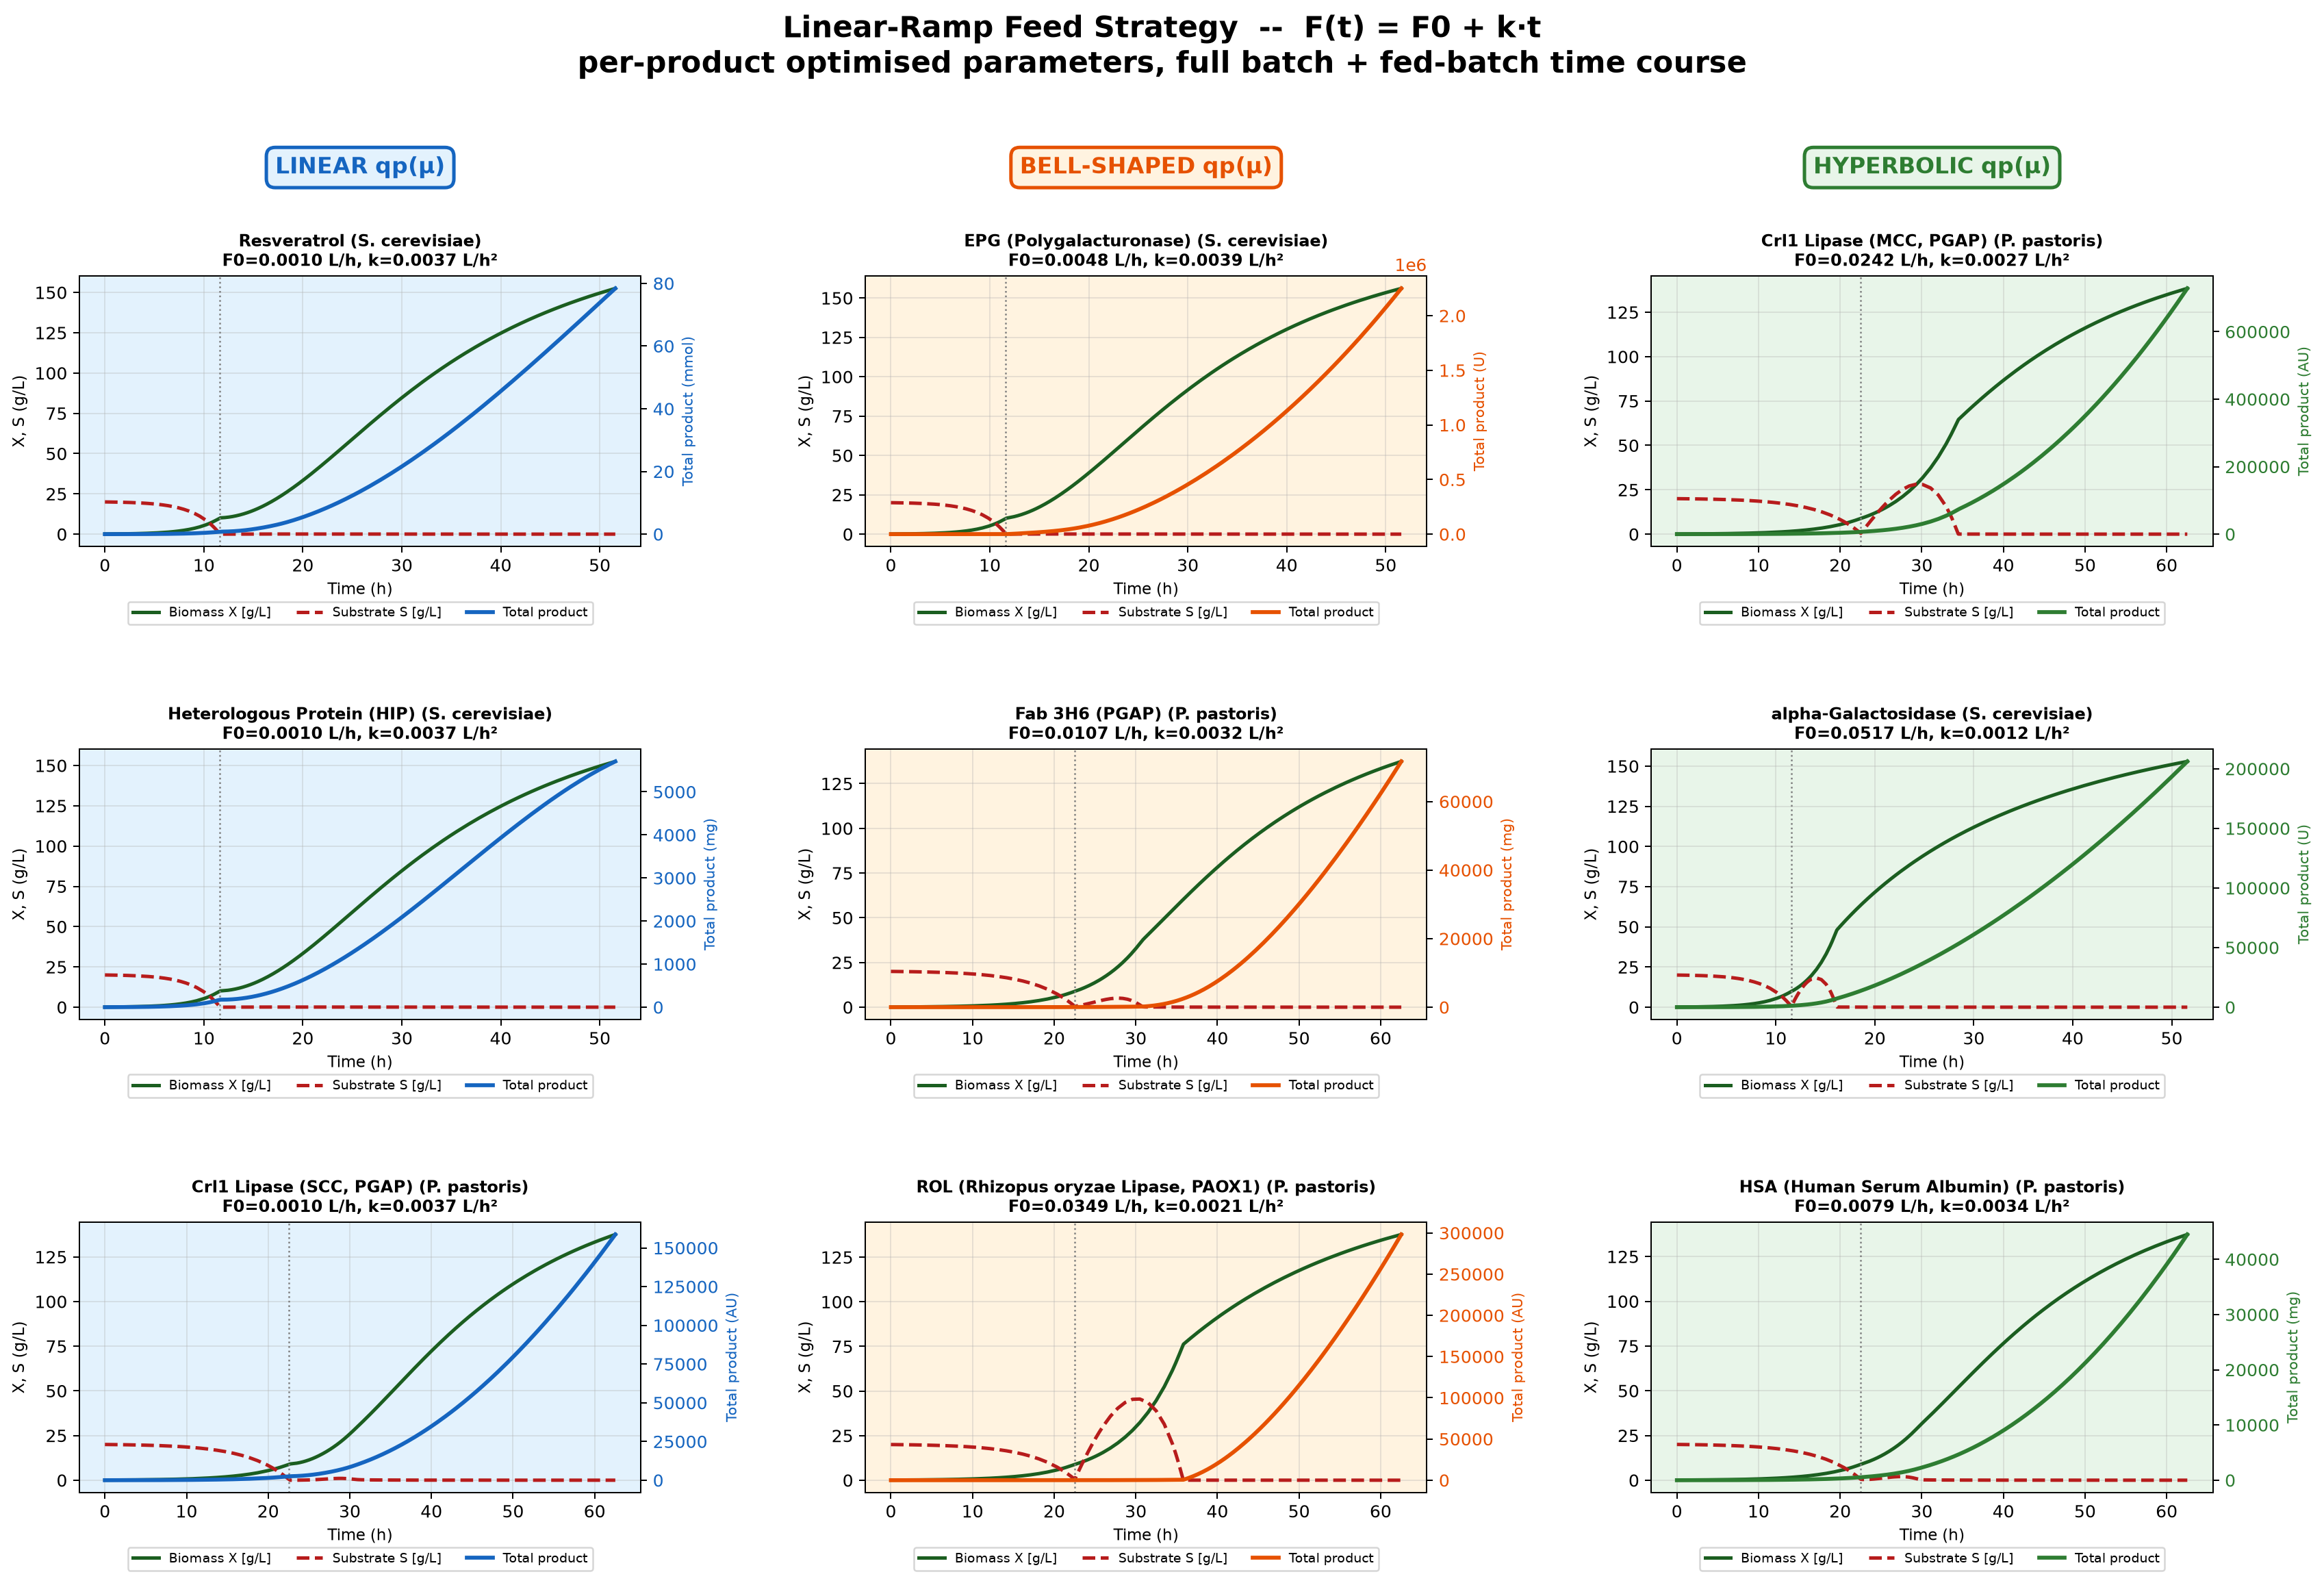
\includegraphics[height=0.72\textheight]{feed_flow_linear_ramp_only.png}
  \end{center}
  \vfill
\end{frame}

% ── Slide 11: Key findings ──────────────────────────────────
\begin{frame}{Key Findings}
  \begin{itemize}
    \item \textbf{Bell-shaped: exponential feed wins.} Holding $\mu$ near the fitted
      $\mu_{opt}$ via an exponential feed matches theory --- and this is also where
      strategy choice matters \textit{most}: a Gaussian $q_p(\mu)$ punishes drifting
      off $\mu_{opt}$ in either direction.
    \item \textbf{Hyperbolic: a gentle linear-ramp feed wins, by tiny margins.} Once
      $\mu$ clears $K_\mu$, $q_p$ is already near $q_p^{max}$ --- almost any
      reasonable strategy is close to optimal. Most forgiving shape to feed for.
    \item \textbf{Linear: exponential feed generally wins} (push $\mu$ as high as the
      data supports), except where the fit never saturates within the sampled
      $\mu$-range --- there, a strategy that can transiently spike $\mu$ higher
      captures slightly more product before the volume budget runs out.
  \end{itemize}
\end{frame}

% ── Slide 12: Emergent result ───────────────────────────────
\begin{frame}{An Emergent Result the Theory Didn't Predict}
  \begin{block}{Time-averaged $\mu$ converges across strategies}
    Within any single dataset, the time-averaged $\mu$ ends up nearly identical
    across all 7 strategies, even though the $F(t)$ curves look very different.
  \end{block}

  \vspace{0.3cm}
  \textbf{Why:} the shared $V_{max}$ ceiling fixes the \textit{total} substrate that
  can ever be delivered, $(V_{max}-V_0)\cdot S_{in}$. Monod growth self-regulates: once
  the system is substrate-limited, $S$ settles into a similar quasi-steady balance
  against consumption regardless of the feed law's shape.

  \vspace{0.3cm}
  So the real lever the optimiser pulls isn't ``a wildly different average $\mu$''
  --- it's \textit{how efficiently the fixed feed budget is spent over time}
  relative to each $q_p(\mu)$ curve's shape.
\end{frame}

% ── Slide 13: Practical takeaway ────────────────────────────
\begin{frame}{Practical Takeaway}
  \begin{columns}[T]
    \begin{column}{0.31\textwidth}
      \begin{block}{Bell-shaped}
        \centering
        \small Invest in a growth-rate controller (exponential feed, or closed-loop
        feedback) --- the payoff for getting the feed law right is the largest here.
      \end{block}
    \end{column}
    \begin{column}{0.34\textwidth}
      \begin{block}{Hyperbolic}
        \centering
        \small A simple, low-maintenance feed (linear ramp, or even constant) is
        close enough --- not worth the operational complexity of active control.
      \end{block}
    \end{column}
    \begin{column}{0.31\textwidth}
      \begin{block}{Linear}
        \centering
        \small Favour exponential feeding to sustain the highest $\mu$ the data
        supports; check for saturation before ruling out short-pulse feeding.
      \end{block}
    \end{column}
  \end{columns}

  \vspace{0.3cm}
  {\small Closes the ``Fed-Batch Models'' roadmap item and starts ``Parameter
  Estimation \& Optimisation.''}
\end{frame}

% ── Slide 14: Web platform update ───────────────────────────
\begin{frame}{Web Platform: Verified End-to-End}
  \begin{columns}[T]
    \begin{column}{0.48\textwidth}
      \textbf{Verified for real} (in the \texttt{bpdd} conda env, real
      assimulo/pygmo):
      \begin{itemize}
        \item[\textcolor{donegreen}{\checkmark}] 485/494 \texttt{pyfoomb} tests pass
        \item[\textcolor{donegreen}{\checkmark}] 39/39 backend API tests pass
        \item[\textcolor{donegreen}{\checkmark}] Clean \texttt{lint}/\texttt{build}
        \item[\textcolor{donegreen}{\checkmark}] Deployed: frontend on Vercel, backend
              on Render
      \end{itemize}
    \end{column}
    \begin{column}{0.48\textwidth}
      \textbf{Bug found \& fixed:}
      \begin{itemize}
        \item \texttt{pygmo.mp\_island}'s worker-pool init calls
              \texttt{signal.signal()}, which crashes when FastAPI runs it on a
              worker thread --- fixed by pre-warming the pool at app startup
              (main thread).
        \item Error toasts used the wrong ARIA role for screen readers --- fixed to
              match the existing status-message convention.
      \end{itemize}
      \vspace{0.15cm}
      {\small Remaining, not fixable in \texttt{pyfoomb} code: the \texttt{bpdd}
      env's pygmo/pagmo build has a broken (un)pickling registry that blocks
      \texttt{estimate\_parallel} on \texttt{mp\_island} --- needs an upstream fix
      or a different build.}
    \end{column}
  \end{columns}
\end{frame}

% ── Slide 15: Roadmap ────────────────────────────────────────
\begin{frame}{Project Roadmap}
  \vspace{-0.1cm}
  \begin{center}
  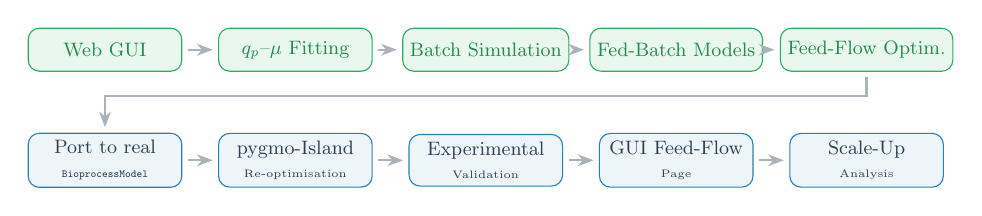
\begin{tikzpicture}[
    scale=0.78, every node/.style={scale=0.78, align=center},
    doneblock/.style={rectangle, rounded corners=4pt, minimum width=2.5cm, minimum height=0.7cm,
      draw=donegreen, fill=donegreen!10, font=\small, text=donegreen!80!black},
    pendblock/.style={rectangle, rounded corners=4pt, minimum width=2.5cm, minimum height=0.7cm,
      draw=accentblue, fill=accentblue!8, font=\small, text=darkcharcoal},
    arr/.style={-{Stealth[length=2mm]}, thick, color=darkcharcoal!40, shorten >=2pt, shorten <=2pt}
  ]
    \node[doneblock] (a1) at (0,0) {Web GUI};
    \node[doneblock] (a2) at (3.1,0) {$q_p$--$\mu$ Fitting};
    \node[doneblock] (a3) at (6.2,0) {Batch Simulation};
    \node[doneblock] (a4) at (9.3,0) {Fed-Batch Models};
    \node[doneblock] (a5) at (12.4,0) {Feed-Flow Optim.};

    \draw[arr] (a1) -- (a2);
    \draw[arr] (a2) -- (a3);
    \draw[arr] (a3) -- (a4);
    \draw[arr] (a4) -- (a5);

    \node[pendblock] (b1) at (0,-1.8) {Port to real\\{\tiny \texttt{BioprocessModel}}};
    \node[pendblock] (b2) at (3.1,-1.8) {pygmo-Island\\{\tiny Re-optimisation}};
    \node[pendblock] (b3) at (6.2,-1.8) {Experimental\\{\tiny Validation}};
    \node[pendblock] (b4) at (9.3,-1.8) {GUI Feed-Flow\\{\tiny Page}};
    \node[pendblock] (b5) at (12.4,-1.8) {Scale-Up\\{\tiny Analysis}};

    \draw[arr] (a5.south) -- ++(0,-0.4) -| (b1.north);
    \draw[arr] (b1) -- (b2);
    \draw[arr] (b2) -- (b3);
    \draw[arr] (b3) -- (b4);
    \draw[arr] (b4) -- (b5);
  \end{tikzpicture}
  \end{center}

  \vspace{0.3cm}
  \begin{columns}[T]
    \begin{column}{0.48\textwidth}
      \textbf{Completed this semester:}
      {\small
      \begin{itemize}
        \item[\textcolor{donegreen}{\checkmark}] Fed-batch $F(t)$ process model, 7 strategies
        \item[\textcolor{donegreen}{\checkmark}] Volume-ceiling bug found \& fixed
        \item[\textcolor{donegreen}{\checkmark}] Web GUI verified against real solvers, deployed
      \end{itemize}
      }
    \end{column}
    \begin{column}{0.48\textwidth}
      \textbf{Planned next:}
      {\small
      \begin{itemize}
        \item[\textcolor{accentblue}{$\circ$}] Re-optimise with real CVode + pygmo islands
        \item[\textcolor{accentblue}{$\circ$}] Validate against experimental fed-batch runs
        \item[\textcolor{accentblue}{$\circ$}] Turn strategies into a ranked GUI page
      \end{itemize}
      }
    \end{column}
  \end{columns}
\end{frame}

% ── Slide 16: Thank You ──────────────────────────────────────
\begin{frame}[plain]
  \vfill
  \begin{center}
    {\LARGE\bfseries\color{darkcharcoal} Thank You}\\[0.6cm]
    {\large\color{accentblue} Questions?}\\[1cm]
    \begin{tabular}{rl}
      \textbf{Student:} & Yashashwi Singhania (23014019) \\
      \textbf{Guide:} & Dr.\ Sharon Mano Pappu J. \\
      \textbf{Lab:} & BPDD, Dept.\ of Biochemical Engineering \\
      \textbf{Institute:} & IIT (BHU) Varanasi \\
    \end{tabular}\\[0.8cm]
    {\small\color{darkcharcoal!60} July 2026}
  \end{center}
  \vfill
\end{frame}

\end{document}
